\subsection{Diferenças sobre linguagens convencionais}
\label{diferencasdsl}

Segundo \citeonline{dslengineering}, o propósito das \gls{DSL} é de atender a um domínio específico, são construídas para resolver uma classe específica de problemas. De outro lado as \gls{GPL} são voltadas aos desenvolvedores para resolver qualquer tipo de problema computável:

\begin{citacao}
As Linguagens de Programação de Uso Geral (GPLs) são um meio para programadores instruírem computadores.Todas podem ser usadas para implementar qualquer coisa computável com uma máquina de Turing. Isso também significa que qualquer coisa expressável com uma linguagem de programação completa de Turing também pode ser expressa em qualquer outra linguagem de programação completa de Turing. Nesse sentido, todas as linguagens de programação são intercambiáveis. \cite{dslengineering}
\end{citacao}

Para \citeonline{ghosh2011dsl}, projetar uma DSL não é uma tarefa tão assustadora quanto projetar uma linguagem de programação de uso geral. Pois tem foco limitado e é restrita apenas ao domínio que está sendo modelado.

Enquanto \gls{GPL} são flexíveis, as \gls{DSL} sacrificam a flexibilidade em benefício da produtividade e da concisão de programas relevantes em um domínio específico. As \gls{GPL}s são utilizadas em domínios maiores e complexos, do outro lado são trabalhados problemas menores e bem definidos \cite{dslengineering}. Algumas dessas diferenças podem ser observadas na  Figura \ref{fig:gplvsdsl}.

\begin{figure}[h!]
\centering

\caption{\textmd{DSL vs GPL}}
\label{fig:gplvsdsl}
\fcolorbox{gray}{white}{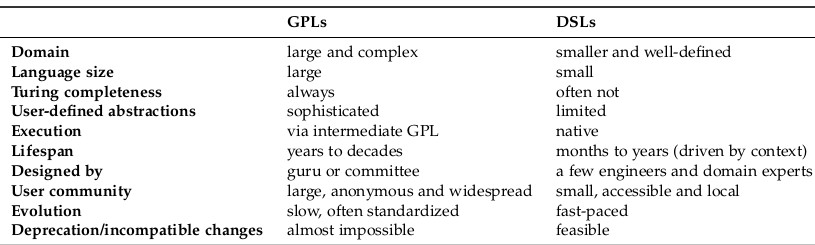
\includegraphics[width=\textwidth]{chapters/fundamentacao/imagens/gplvsdsl.jpg}}

\par\medskip\textbf{Fonte:} \citeonline{dslengineering}. \par\medskip
\end{figure}


Existem situações em que, usuários sem habilidades de programação, precisam injetar regras no sistema, ou definir condições de modo que possam atender uma funcionalidade ou requisito necessário, porém, não é viável ensina-los conceitos básicos de linguagens de programação. A configuração usando uma linguagem específica de domínio pode ser uma alternativa para resolver estas situações \cite{novak2010easy}.  

No entanto, como em qualquer desenvolvimento de modelagem de software, existem desafios a serem considerados para tomada de decisão sobre adoção \gls{DSL}s no desenvolvimento de software. Na Seção \ref{beneficiosdsl}, serão pontuados alguns desses desafios e vantagens encontrados na literatura.

\subsection{Vantagens e Desafios no desenvolvimento de DSLs}
\label{beneficiosdsl}



\subsection{Ferramentas de construção de DSL}
\label{ferramentasdsl}